\documentclass[a4paper,12pt]{article} % declaration

% packages

\usepackage[utf8]{inputenc}
\usepackage{amsmath}
\usepackage{amsthm}
\usepackage{amsfonts}
\usepackage{color}
\usepackage{graphicx}

%\def\pgfsysdriver{pgfsys-dvipdfmx.def}
\usepackage{tikz}

\newtheorem{definition}{Definition}[section]
\newtheorem{theorem}{Theorem}[section]
\newtheorem{proposition}{Proposition}[section]
\newtheorem{lemma}[theorem]{Lemma}
\newtheorem{corollary}[theorem]{Corollary}
\newtheorem{example}{Examples}
\title{Limit}
\author{Guoning Wu}
\begin{document}
\tableofcontents
\setcounter{tocdepth}{2}
\listoffigures
\listoftables
\maketitle
%======================================================
In discussing the various aspects of the concept of a real number we 
remarked in particular that in measuring real physical quantities 
we obtain sequences of approximate values with which one must then 
work. Such a state of affairs immediately raises at least the following 
three questions:
\begin{enumerate}
    \item What relation does the sequence of approximations so obtained 
        have to the quantity being measured?
    \item How are operations on the approximate values connected with the 
        same operations on the exact values?
    \item How can one determine from a sequence of numbers whether it can
        be a sequence of arbitrarily precise approximations of the values 
        of some quantity?
\end{enumerate}

\section{The Limit of a Sequence}
\subsection{Definitions and Examples}
We recall the following definition.
\begin{definition}
    A function $f: \mathbb{N} \to X$ whose domain of definition is the set of 
    natural numbers is called a \textit{sequence}.
\end{definition}

The values $f(n)$ of the function $f$ are called the terms of the sequence. We 
denote $x_n  := f(n)$. In this connection the sequence itself is denoted $\{x_n\}$,
and also written as $x_1, x_2, \cdots , x_n \cdots $. It is called a sequence in $X$.

The element $x_n$ is called the \textit{nth term of the sequence}.

\begin{definition}
    A number $A \in \mathbb{R}$ is called the \textit{limit of the numerical sequence}
     $\{x_n\}$ if for every neighborhood $V(A)$ of $A$ there exists an index $N$
    (depending on $V(A)$) such that all terms of the sequence having index larger 
    than $N$ belong to the neighborhood $V(A)$.
\end{definition}

We now write these formulations of the definitions of a limit in the 
language of symbolic logic.
\[\lim_{n \to \infty} x_n = A := \forall V(A), \exists N \in \mathbb{N}, \forall n>N, x_n \in V(A)\],
and respectively
\[\lim_{n \to \infty } = A := \forall \epsilon >0, \exists N\in \mathbb{N}, \forall n>N, |x_n - A|<\epsilon\].
\begin{definition}
    If $\displaystyle \lim_{n \to \infty} x_n = A$, we say the sequence $\{x_n\}$ 
    converges to $A$ and writes $x_n \to A$ as $n \to \infty$.
\end{definition}

A sequence having a limit is said to be convergent. A sequence that does not 
have a limit is said to be divergent.

Let us consider some examples.
\begin{example}
    $\displaystyle \lim_{n \to \infty} \frac{1}{n} = 0.$
\end{example}
\begin{example}
    $\displaystyle \lim_{n \to \infty} \frac{n+1}{n} = 1.$
\end{example}
\begin{example}
    $\displaystyle \lim_{n \to \infty} \left( 1+\frac{(-1)^n}{n}\right) = 1.$
\end{example}
\begin{example}
    $\displaystyle \lim_{n \to \infty} \frac{\sin n}{n} = 0.$
\end{example}
\begin{example}
    $\displaystyle \lim_{n \to \infty} \frac{1}{q^n} = 0, {\rm if } |q|>1.$
\end{example}
\begin{example}
    The sequence $1, 2, \frac{1}{3}, 4, \frac{1}{5}, \cdots$ whose $n$
    term is $\displaystyle x_n = n^{(-1)^n}$ is divergent. 
\end{example}
\begin{example}
    The sequence $1, -1, 1, -1, \cdots$ for which $x_n = (-1)^n$, has no limit.
\end{example}

\subsection{Properties of the Limit of a Sequence}
\subsubsection{General Properties}
\begin{definition}
    If there exists a number $A$ and an index $N$ such that $x_n = A$
    for all $n>N$, the sequence $\{x_n\}$ will be called ultimately 
    constant.
\end{definition}
\begin{definition}
    A sequence $\{x_n\}$ is bounded if there exists $M$ such that $|x_n| < M$
    for all $n \in M$.
\end{definition}

\begin{theorem}
    1) An ultimately constant sequence converges.

    2) Any neighborhood of the limit of a sequence contains all but 
    a finite number of terms of the sequence.

    3) A convergent sequence cannot have two different limits.

    4) A convergent sequence is bounded.
\end{theorem}

\subsubsection{Passage to the Limit and the Arithmetic Operation}
\begin{definition}
    If $\{x_n\}$ and $\{y_n\}$ are two numerical sequences,their sum, 
    product, and quotient are the sequences
    \[\{x_n+y_n\}, \{x_n \cdot y_n\}, \left\{\frac{x_n}{y_n}\right\}\]
\end{definition}
The quotient, of course, is defined only when $y_n\ne 0$ for all $n \in N$.

\begin{theorem}
    Let $\{x_n\}$ and $\{y_n\}$ be numerical sequences. If $\displaystyle \lim_{n\to \infty}
    x_n =A$ and $\displaystyle \lim_{n\to \infty} y_n =B$, then 

    {\rm a)} $\displaystyle \lim_{n\to \infty}\left(x_n+y_n \right) = A+B$.
    
    {\rm b)} $\displaystyle \lim_{n\to \infty}\left(x_n \cdot y_n \right) = A \cdot B$.

    {\rm c)} $\displaystyle \lim_{n\to \infty}\left(x_n \setminus y_n \right) = A \setminus B$,
    provided that $y_n \ne 0 (n=1,2,\cdots,),B\ne0$.
\end{theorem}

\subsubsection{Passage to the Limit and Inequalities}
\begin{theorem}
    {\rm a) } Let $\{x_n\}$ and $\{y_n\}$ be numerical sequences. If $\displaystyle \lim_{n\to \infty}
    x_n =A$ and $\displaystyle \lim_{n\to \infty} y_n =B$. If $A < B$, then there exists an 
    index $N \in \mathbb{N}$ such that $x_n < y_n$  for all $n > N$.
\end{theorem}
\begin{corollary}
    Suppose $\displaystyle \lim_{n\to \infty}
    x_n =A$ and $\displaystyle \lim_{n\to \infty} y_n =B$.
    If there exists $N$ such that for all $n > N$ we have 

    {\rm a)} $x_n > y_n$, then $A \ge B$.

    {\rm b)} $x_n \ge y_n$, then $A \ge B$.

    {\rm c)} $x_n > B$, then $A \ge B$.

    {\rm d)} $x_n \ge B$, then $A \ge B$.
\end{corollary}

\subsubsection{Questions Involving the Existence of the Limit of a Sequence}
\paragraph{{\rm \textbf{ a. The Cauchy Criterion}}}
\begin{definition}
    A sequence ${x_n}$ is called a \textit{fundamental or Cauchy} sequence 
    if for any $\epsilon > 0$ there exists an index $N \in \mathbb{N}$
    such that $|x_m - x_n| < \epsilon$ whenever $n > N$ and $m > N$.
\end{definition}
\begin{theorem}{(Cauchy's convergence criterion)}
    A numerical sequence converges if and only if it is a Cauchy sequence.
\end{theorem}
\begin{proof}
    \[a_n := \inf_{k\ge n} x_k\]
    \[b_n:= \sup_{k\ge n} x_k\]
    Since $a_n \le b_n$, 
    \[a_n = \inf_{k\ge n} x_k \le x_k \le \sup_{k\ge n} x_k = b_k\]
    \[a_n \le A \le b_n\]
    \[\left|x_k - A\right| \le b_n - a_n\]
\end{proof}
\begin{example}
    The sequence $(-1)^n, n = 1,2,\cdots$ has no limit.
\end{example}
\begin{example}
    Let \[x_1 = 0, x_2 = 0.\alpha_1, x_3 = 0.\alpha_1\alpha_2, \cdots, x_n = 0.\alpha_1\alpha_2\cdots\alpha_n, \cdots\]
    be a sequence of finite binary fractions in which each successive
    fraction is obtained by adjoining a 0 or a 1 to its predecessor. 
    Such a sequence always converges.
\end{example}

\begin{example}
    Suppose $\{x_n\}$ satisfies $\displaystyle |x_{n+1} - x_{n}| \le k|x_n - x_{n-1}
    |, 0 < k < 1, n=1,2,\cdots,$
    then $\{x_n\}$ converges.
\end{example}

\paragraph{{\rm \textbf{b. Some Criterions for the Existence of the Limit 
of Sequences}}}
\begin{definition}
    A sequence ${x_n}$ is increasing if $x_n < x_{n+1}$ for all $n \in \mathbb{N}$,
    nondecreasing if $x_n \le x_{n+1}$ for all $n \in \mathbb{N}$,
    nonincreasing if $x_n \ge x_{n+1}$ for all $n \in \mathbb{N}$, and 
    decreasing if $x_n > x_{n+1}$ for all $n \in \mathbb{N}$.
    Sequences of these four types are called monotonic sequences.
\end{definition}
\begin{definition}
    A sequence ${x_n}$ is bounded above if there exists a number $M$
    such that $x_n < M$ for all $n \in \mathbb{N}$.
\end{definition}
\begin{theorem}{(Weierstrass)}
    In order for a non-decreasing sequence to have a limit it is 
    necessary and sufficient that it is bounded above.
\end{theorem}
\begin{proof}
    Let $s = \sup_{n\in \mathbb{N}}x_n$, prove that 
    \[\lim_{n \to \infty}x_n = s \]
\end{proof}

\begin{example}
    \[\lim_{n \to \infty} \frac{n}{q^n} = 0, q>1\]
\end{example}
\begin{corollary}
    \[\lim_{n \to \infty} \sqrt[n]{n} = 1\]
\end{corollary}

\begin{example}
    \[\lim_{n \to \infty} \sqrt[n]{a} = 1,\text{for any } a>0\]
\end{example}

\begin{example}
    \[
        \lim_{n \to \infty} \frac{q^n}{n!} = 0.
        \]
\end{example}
\begin{example}
    \[\lim_{n \to \infty} 1+\frac{1}{2}+\frac{1}{3}+\cdots+\frac{1}{n}-\ln n \]
\end{example}

\begin{example}
    \emph{Suppose} $x_1 > 0, x_{n+1} = 1+\frac{x_n}{1+x_n}, n = 1,2,\cdots$.
    \emph{Find the limit of} $x_n$.
\end{example}

\begin{example}
    \emph{Suppose} $x_1 = \sqrt{a}, x_2 = \sqrt{a+x_1}, \cdots, x_n = \sqrt{a + x_{n-1}}, \cdots$, 
    for $a \in \mathbb{R}^+.$
    \emph{Find the limit} $\lim_{n \to \infty} x_n$.
\end{example}

\begin{example}
    \emph{The Fibonacci sequence is: }
    \[
        a_1 = 1, a_2 = 1, a_3 = a_1 + a_2, \cdots, a_{n+1} = a_n + a_{n-1}, \cdots
        \]
    \emph{if we take }
    $\displaystyle b_n = \frac{a_{n+1}}{a_n}, n = 1,2,\cdots$.
    \emph{Then find the} $\displaystyle \lim_{n \to \infty} b_n$.
\end{example}

\paragraph{{\rm \textbf{c. The Number e }}}
\begin{example}
    Let us prove that the limit $\displaystyle \lim_{n \to \infty}\left(1+\frac{1}{n}\right)^n $ exists.
\end{example}
In this case the limit is a number denoted by the letter e, after Euler
\footnote{\textbf{Leonhard Euler:}(1707-1783) was a Swiss mathematician, 
physicist, astronomer, logician and engineer who was made important and 
influential discoveries in many branches of mathematics like infinitesimal 
calculus and graph theory while also making pioneering contributions to 
several branches such as topology and analytic number theory. He is also
introduced much of the modern mathematical terminology and notation, particularly 
for mathematical analysis, such as notion of a mathematical function. He is also 
known for his work in mechanics, fluid dynamics, optics, astronomy, and music theory.}.
This number is just as central to analysis as the number 1 to arithmetic 
or $\pi$ to geometry. We begin by verifying the following inequality, 
sometimes called Jakob Bernoulli's inequality. \footnote{Jakob Bernoulli 
(1654-1705) - Swiss mathematician, a member of the famous Bernoulli 
family of scholars. He was one of the founders of the calculus of 
variations and probability theory.}

\[(1+\alpha)^n \ge 1 + n\alpha \text{ for } n \in \mathbb{N} \text{ and } \alpha > -1 \]
\begin{proof}
    The assertion is true for $n=1$. If it holds for $n \in \mathbb{N}$,
    then it must hold for $n+1$, since we have 
    \[(1+\alpha)^{n+1}=(1+\alpha)(1+\alpha)^n\ge(1+\alpha)(1+n\alpha)\ge1+(n+1)\alpha\]
\end{proof}
\graphicspath{{../Figs/}}
\begin{figure}[htbp]
    \centering
    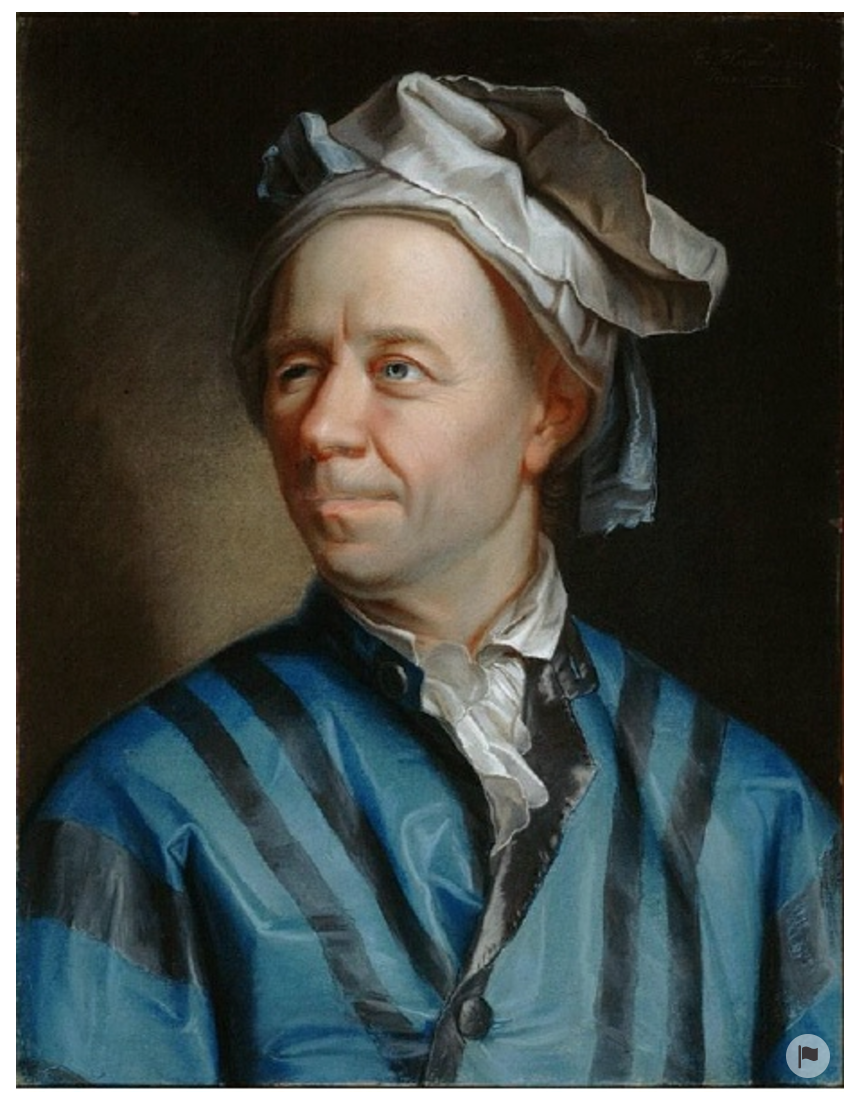
\includegraphics[width=0.4\textwidth]{Euler.png}
    \caption{Leonhard Euler.}
    \label{fig:fig1}
\end{figure}


We now show that the sequence $\displaystyle y_n = \left(1+\frac{1}{n}\right)^{n+1}$
is decreasing.
\begin{proof}
    \[
    \begin{split}
        \frac{y_{n-1}}{y_n} &=\frac{\left(1+\frac{1}{n-1}\right)^n}{\left(1+\frac{1}{n}\right)^{n+1}}
         = \frac{n^{2n}}{(n^2-1)^n}\cdot\frac{n}{n+1} = \left(1+\frac{1}{n^2-1}\right)^2
         \cdot\frac{n}{n+1}\\
        & \ge \left(1+\frac{n}{n^2-1}\right)\frac{n}{n+1} > \left(1+\frac{1}{n}\right)
        \frac{n}{n+1} = 1
    \end{split}
    \]
Since the terms of the sequence are positive, the limit 
    $\displaystyle \lim_{n \to \infty} \left(1+\frac{1}{n}\right)^{n+1}$
    exists. But we then have 
    \[ \begin{split}
        \lim_{n \to \infty} &\left(1+\frac{1}{n}\right)^n = \lim_{n \to \infty} \left(1+\frac{1}{n}\right)^{n+1}
        \left(1+\frac{1}{n}\right)^{-1}  \\
        & = \lim_{n \to \infty}\left(1+\frac{1}{n}\right)^{n+1} 
        \lim_{n \to \infty} \frac{1}{1+\frac{1}{n}}=
        \lim_{n \to \infty}\left(1+\frac{1}{n}\right)^{n+1} 
    \end{split}
    \]
\end{proof}

\begin{definition}
    \[e:= \lim_{n \to \infty} \left(1+\frac{1}{n}\right)^n.\]
\end{definition}

\paragraph{{\rm \textbf{The Mathematical Constant e.}}}
The number e is a mathematical constant that is the base of the natural 
logarithm: the unique number whose natural logarithm is equal to one. 
It is approximately equal to 2.71828, and is the limit of (1 + 1/n)n 
as n approaches infinity, an expression that arises in the study of compound 
interest. It can also be calculated as the sum of the infinite series.
\[
    e= \sum \limits _{n=0}^{\infty }\dfrac {1}{n!}
     =\frac {1}{1}+\frac {1}{1}+\frac {1}{1\cdot 2}+\frac {1}{1\cdot 2\cdot 3}+\cdots .
\]
Sometimes called Euler's number after the Swiss mathematician Leonhard Euler, 
e is not to be confused with $\gamma$, the Euler–Mascheroni constant, sometimes called 
simply Euler's constant. The number e is also known as Napier's constant, 
but Euler's choice of the symbol e is said to have been retained in his honor.
The constant was discovered by the Swiss mathematician Jacob Bernoulli while 
studying compound interest.

The number e is of eminent importance in mathematics, alongside 0, 1, $\pi$ and i. 
All five of these numbers play important and recurring roles across mathematics,
and are the five constants appearing in one formulation of Euler's identity. 
\[
    e^{i\pi} + 1 = 0.
    \]
where e is Euler's number, the base of natural logarithms,
i is the imaginary unit, which satisfies $i^2 = -1$, and
$\pi$ is pi, the ratio of the circumference of a circle to its diameter.

Euler's identity is named after the Swiss mathematician Leonhard Euler. 
It is considered to be an example of mathematical beauty.
Like the constant $\pi$, e is irrational: it is not a ratio of integers. Also 
like $\pi$, e is transcendental: it is not a root of any non-zero polynomial 
with rational coefficients. The numerical value of e truncated to 50 decimal places is


\textbf{2.718281828459045235360287471352662497757247093699.}


The first references to the constant were published in 1618 in the table of 
an appendix of a work on logarithms by John Napier. However, this did not contain 
the constant itself, but simply a list of logarithms calculated from the constant. 
It is assumed that the table was written by William Oughtred. The discovery of the 
constant itself is credited to Jacob Bernoulli in 1683, who attempted to find the 
value of the following expression (which is in fact e):
\[
    \lim _{n\to \infty }\left(1+\frac {1}{n}\right)^{n}.
\]
The first known use of the constant, represented by the letter b, was in correspondence 
from Gottfried Leibniz to Christiaan Huygens in 1690 and 1691. Leonhard Euler introduced 
the letter e as the base for natural logarithms, writing in a letter to 
Christian Goldbach of 25 November 1731. Euler started to use the letter e 
for the constant in 1727 or 1728, in an unpublished paper on explosive 
forces in cannons, and the first appearance of e in a publication was 
in Euler's Mechanica (1736). While in the subsequent years some researchers 
used the letter c, e was more common and eventually became the standard.

\begin{example}
    \emph{Find the limit of }
    \[
        \lim_{n \to \infty}\left\{1 + \frac{1}{2} + \frac{1}{3} + \cdots + \frac{1}{n} - \ln n \right\}
        \]
    \label{ex:ex1}
\end{example}

The limit of the sequence of Example~\ref{ex:ex1} is called the Euler–Mascheroni 
constant.The numerical value of the Euler–Mascheroni constant, to 50 decimal 
places, is:

\textbf{0.57721566490153286060651209008240243104215933593992….}

\paragraph{{\rm \textbf{The Euer-Mascheroni Constant.}}}
The Euler–Mascheroni constant (also called Euler's constant) is a mathematical 
constant recurring in analysis and number theory, usually denoted by the 
lowercase Greek letter gamma ($\gamma$).

It is defined as the limiting difference between the harmonic series and 
the natural logarithm:
\[
    \begin{aligned}
        \gamma &=\lim_{n\to \infty }\left(-\ln n+\sum _{k=1}^{n}\frac {1}{k}\right)\\
    &=\int _{1}^{\infty }\left(\frac {1}{\lfloor x\rfloor }-\frac {1}{x}\right)
    \,dx.
    \end{aligned}
    \]
Here, $\lfloor \rfloor$ represents the floor function.

The constant first appeared in a 1734 paper by the Swiss mathematician 
Leonhard Euler, titled De Progressionibus harmonicis observationes 
(Eneström Index 43). Euler used the notations C and O for the constant. 
In 1790, Italian mathematician Lorenzo Mascheroni used the notations A 
and a for the constant. The notation $\gamma$ appears nowhere in the writings 
of either Euler or Mascheroni, and was chosen at a later time perhaps 
because of the constant's connection to the gamma function. For example,
the German mathematician Carl Anton Bretschneider used the notation 
$\gamma$ in 1835 and Augustus De Morgan used it in a textbook published 
in parts from 1836 to 1842.

\begin{example}
    \[
        \lim_{n \to \infty}\left(\frac{1}{n+1} + \frac{1}{n+2} + \cdots + \frac{1}{2n}\right)
        = \ln 2.
\]\end{example}

\begin{example}
    \[
        \lim_{n \to \infty}\left(1 - \frac{1}{2} + \frac{1}{3} + \cdots + 
        (-1)^{n+1}\frac{1}{n}\right) = \ln 2.
    \]
\end{example}

\paragraph{{\rm \textbf{d. Subsequences and Partial Limits of a Sequence}}}
\begin{definition}
    If $x_1, x_2, \cdots, x_n, \cdots$ is a sequence and $n_1 < n_2 < \cdots <n_k < \cdots$
    an increasing sequence of natural numbers, then the sequence 
    $x_{n_1}, x_{n_2}, \cdots, x_{n_k} \cdots$ is a subsequence of the sequence ${x_n}$.
\end{definition}
\begin{lemma}{(Bolzano-Weierstrass)}
    Every bounded sequence of real numbers contains a convergent subsequence.
\end{lemma}

\begin{definition}
    We shall write $x_n \to +\infty$ and say that the sequence ${x_n}$
    tends to positive infinity if for each number $c$ there exist 
    $N \in \mathbb{N}$ such that $x_n > c$ for all $n > N$.
\end{definition}

\begin{lemma}
    From each sequence of real numbers one can extract either a convergent 
    subsequence or a subsequence that tends to infinity.
\end{lemma}

Let $x_k$ be an arbitrary sequence of real numbers. If it is bounded below,
one can consider the sequence $\displaystyle i_n = \inf_{k\ge n} x_k$.
\begin{definition}
    The number $\displaystyle l = \lim_{n \to \infty} \inf_{k \ge n}x_k$
    is called the inferior limit of the sequence ${x_n}$ and denoted 
    $\displaystyle \varliminf_{k \to \infty} x_k$
    or $\displaystyle \lim \inf_{k \to \infty} x_k$. If$i_n \to +\infty$,
    it is said that the inferior limit of the sequence equals positive 
    infinity, and we write $\displaystyle \varliminf_{k \to \infty} x_k 
    = +\infty$. If the original sequence ${x_n}$ is not bounded below, the we 
    shall have $i_n = \inf_{k \ge n} x_k = -\infty$ for all $n$. In that case 
    we say that the inferior limit of the sequence equals negative 
    infinity and write $\displaystyle \varliminf_{k \to \infty} x_k
    = -\infty$.
\end{definition}

\begin{definition}
    \[\varlimsup_{k \to \infty}x_k = \lim_{n \to \infty}
    \sup_{k \ge n}x_k\]
\end{definition}

\begin{example}
    $x_k = (-1)^k, k \in \mathbb{N}$.
    \[\varliminf_{k \to \infty} x_k = -1\]
    \[\varlimsup_{k \to \infty} x_k = 1\]
\end{example}

\begin{example}
    $\displaystyle x_k = k^{(-1)^k}$.
    \[ \varliminf_{k \to \infty} k^{(-1)^k} = \lim_{n \to \infty} 
    \inf_{k \ge n} k^{(-1)^k}= \lim_{n \to infty} 0 = 0\]
    \[ \varlimsup_{k \to \infty} k^{(-1)^k} = \lim_{n \to \infty} 
    \sup_{k \ge n} k^{(-1)^k}= \lim_{n \to \infty} +\infty = +\infty\]
\end{example}

\begin{example}
    $x_k = k, k \in \mathbb{N}$.
    \[ \varliminf_{k \to \infty} k = \lim_{n \to \infty} 
    \inf_{k \ge n} k= \lim_{n \to \infty} n = +\infty\]
    \[ \varlimsup_{k \to \infty} k = \lim_{n \to \infty} 
    \sup_{k \ge n} k = \lim_{n \to \infty} +\infty = +\infty\]
\end{example}

\begin{example}
    $\displaystyle x_k = \frac{(-1)^k}{k}, k \in \mathbb{N}$.
    \[ \varliminf_{k \to \infty} k = \lim_{n \to \infty} 
    \inf_{k \ge n} \frac{(-1)^k}{k}= 0\]
    \[ \varlimsup_{k \to \infty} k = \lim_{n \to \infty} 
    \sup_{k \ge n} \frac{(-1)^k}{k} = 0\]
\end{example}

\begin{example}
    $\displaystyle x_k = -k^2,k \in \mathbb{N}$
   \[ \varliminf_{k \to \infty} (-k^2) = \lim_{n \to \infty} 
    \inf_{k \ge n} (-k^2)= -\infty\]
    \[ \varlimsup_{k \to \infty} (-k^2) = \lim_{n \to \infty} 
    \sup_{k \ge n} (-k^2) = -\infty\]
\end{example}

\begin{example}
    $x_k = (-1)^kk, k \in \mathbb{N}$
    \[ \varliminf_{k \to \infty} ((-1)^kk) = \lim_{n \to \infty} 
    \inf_{k \ge n} ((-1)^kk)= -\infty\]
    \[ \varlimsup_{k \to \infty} ((-1)^kk) = \lim_{n \to \infty} 
    \sup_{k \ge n} ((-1)^kk) = \infty\]
\end{example}

\begin{definition}
    A number (or the symbol $\infty$ or $-\infty$) is called a partial limit 
    of a sequence, if the sequence contains a subsequence converging 
    to that number.
\end{definition}

\begin{proposition}
    The inferior and superior limits of a bounded sequence 
    are respectively the smallest and the largest partial 
    limits of the sequence.
\end{proposition}

\begin{proposition}
    For any sequence, the inferior limit is the smallest of its 
    partial limits and the superior limit is the largest of its 
    partial limits.
\end{proposition}

\begin{corollary}
    A sequence has a limit or tends to negative or positive infinity 
    if and only if its inferior and superior limits are same.
\end{corollary}

\begin{corollary}
    A sequence converge if and only if every subsequence of it converge.
\end{corollary}

\paragraph{{\rm \textbf{e. Stolz Theorem}}}

\begin{theorem}
    Suppose $\{y_n\}$ is increasing and tends to $+\infty$, and 
    \[\lim_{n \to \infty} \frac{x_n - x_{n-1}}{y_n - y_{n-1}} = a (+\infty, -\infty),\]
    then 
    \[\lim_{n \to \infty} \frac{x_n}{y_n} = a.\]
\end{theorem}

\begin{example}
    \[\lim_{n \to \infty} \frac{1^k+2^2+\cdots+n^k}{n^{k+1}}\]
\end{example}

\begin{example}
    Suppose $\displaystyle \lim_{n \to \infty} a_n = a$, find
    \[\lim_{n \to \infty} \frac{a_1+2a_2+\cdots+na_n}{n^{^2}}\]
\end{example}
\subsubsection{Elementary Facts about Series}
\paragraph{{\rm \textbf{a. The Sum of a Series and the Cauchy Criterion for 
Convergence of a Series}}}
We wish to give a precise meaning to the expression $a_1 + a_2 + \cdots + \cdots,$
which expresses the sums of all the terms of the sequence $\{a_n\}$.

\section{The Limit of a Function}
\subsection{Definitions and Examples}
Let $E$ be a subset of $\mathbb{R}$ and $a$ a limit point of $E$.
Let $f: E \to \mathbb{R}$ be a real-valued function defined on $E$.

\begin{definition}
    We shall say (following Cauchy) that the function $f: E \to \mathbb{R}$ 
    tends to $A$ as $x$ tends to $a$, or that $A$ is the limit of $f$ as $x$ 
    tends to $a$, if for every $\epsilon > 0$ there exist $\delta > 0$ 
such that $|f(x) - A| < \epsilon$ for every $x \in E$ such that $0 < |x - a| < \delta.$
\end{definition}

In logical symbolism these condition are written as 
\[\forall \epsilon > 0, \exists \delta > 0, \forall x \in E \text{ and } 
0 < |x - a| < \delta, \Rightarrow |f(x) - A| < \epsilon \]

\begin{example}
    Let $E = \mathbb{R} \setminus 0$, and $\displaystyle f(x) = x\sin \frac{1}{x}$. We 
    shall verify that \[ \lim_{E \ni x \to 0} x\sin \frac{1}{x} = 0.\]
\end{example}

\begin{definition}
    A deleted neighborhood of a point is a neighborhood of the point 
    from which the point itself has been removed.
\end{definition}

\begin{definition}
    \[\lim_{E \ni x \to a} f(x) = A := \forall V_{\mathbb{R}}(A), \exists 
    \mathring{U}_E(a) \Rightarrow f\left(\mathring{U}_E(a)\right)
    \subset V_R(A).\]
\end{definition}

\begin{example}
    \[
        \lim_{x \to 0} e^x = 1
        \]
\end{example}
\begin{example}
    \[
        \lim_{x \to 2} x^2 = 4
        \]
\end{example}

\begin{example}
    The function 
    \[
        \mbox{sgn} x = \left\{\begin{array}{rcl} 1 & \mbox{if} & x > 0 \\
                                                0 & \mbox{if} & x = 0 \\
                                               -1 & \mbox{if} & x < 0 \\
                             \end{array} \right.
    \]
is defined on the whole line. We shall show that it has no limit 
as $x$ tends to 0.
\end{example}
The nonexistence of this limit is expressed by 
\[
    \forall A \in \mathbb{R}, \exists V(A), \forall \mathring{U}(0) \Rightarrow 
    \exists x \in \mathring{U}(0), f(x) \notin V(A).
\]

\begin{example}
    The function 
    \[
        f(x) = \sin \frac{1}{x}
    \]
has no limit as $x \to 0$
\end{example}

\begin{proposition}
    The relation $\displaystyle \lim_{E \ni x \to a} f(x) = A$ holds if and 
    only if for every sequence $\{x_n\}$ of points $x_n \in E \setminus a $ 
    converging to $a$, the sequence $\{f(x_n)\}$ converges to $A$.
\end{proposition}

\subsection{Properties of the Limit of a Function}
We now establish a number of properties of the limit of a function 
that are constantly being used. Many of them are analogous to the 
properties of the limit of a sequence that have already established.

We call the reader's attention to the fact that, in order to establish 
the properties of the limit of a function, we need only two properties 
of deleted neighborhoods of a limit point of a set:

\begin{enumerate}
    \item $\displaystyle \mathring{U}_E(a) \ne \emptyset$, the deleted neighborhood 
    of the point in $E$ is non-empty.
\item $\displaystyle \forall\mathring{U}_{E_1}(a), \forall\mathring{U}_{E_2}(a),
        \exists\mathring{U}_E(a) \Rightarrow \mathring{U}_E(a) \subset 
        \mathring{U}_{E_1}(a) \cap \mathring{U}_{E_2}(a).$
\end{enumerate}

\paragraph{{\rm \textbf{a. General Properties of the Limit of a Function}}}
\begin{definition}
    A function $f: E \to \mathbb{R}$ assuming only one value is called constant.
    A function $f: E \to \mathbb{R}$ is called ultimately constant as 
    $E \ni x \to a$ if it is constant in some deleted neighborhood $\displaystyle 
    \mathring{U}_E(a)$, where $a$ is a limit point of $E$.
\end{definition}

\begin{definition}
    A function $f: E \to \mathbb{R}$ is bounded, bounded above, or bounded 
    below respectively if there is a number $C \in \mathbb{R}$ such that 
    $\displaystyle \left|f(x)\right| < C$, $f(x) < C$ or $C < f(x)$, for all 
    $x \in E$.
\end{definition}

\begin{example}
    The function $\displaystyle f(x) = \left(\sin \frac{1}{x} + x \cos \frac{1}{x}\right)$
    defined by this formula for $x \ne 0$ is not bounded on its domain of 
    definition, but it is ultimately bounded as $x \to 0$.
\end{example}

\begin{theorem}
    \begin{enumerate}
        \item $f: E \to \mathbb{R}$ is ultimately the constant $A$ as 
            $ \displaystyle E \ni 
            x \to a \Rightarrow \lim_{E \ni x \to a} = A$
        \item $ \displaystyle \lim_{E \ni x \to a} = A \Rightarrow 
            f: E \to \mathbb{R}$ is ultimately bounded as $E \ni x \to a$
        \item $ \displaystyle \lim_{E \ni x \to a} = A_1 \wedge  
            \lim_{E \ni x \to a} = A_2 \Rightarrow A_1 = A_2 $
    \end{enumerate}
\end{theorem}

\paragraph{{\rm \textbf{b. Passage to Limit and Arithmetic Operations}}}
\begin{definition}
    If two numerical-valued functions $f: E \to \mathbb{R}$ and $g: E \to \mathbb{R}$ 
    have a common domain of definition $E$, their sum, product and quotient 
    are respectively the functions defined on the same set by the 
    following formulas:
    \[
        \left(f+g\right)(x) := f(x) + g(x),
        \]
    \[
        \left(f\cdot g\right)(x) := f(x)\cdot g(x),
        \]
    \[
        \left(\frac{f}{g}\right)(x) := \frac{f(x)}{g(x)}.
        \]
\end{definition}

\begin{proposition}
    \begin{enumerate}
        \item If $\displaystyle \alpha: E \to \mathbb{R}$ and $\displaystyle 
            \beta: E \to \mathbb{R}$ are infinitesimal functions as 
            $\displaystyle E \ni x \to a$, then their sum $\alpha + 
            \beta: E \to \mathbb{R}$ also infinitesimal as $E \ni x \to a$.

        \item If $\displaystyle \alpha: E \to \mathbb{R}$ and $\displaystyle 
            \beta: E \to \mathbb{R}$ are infinitesimal functions as 
            $\displaystyle E \ni x \to a$, then their product $\alpha \cdot 
            \beta: E \to \mathbb{R}$ also infinitesimal as $E \ni x \to a$.
        \item If $\displaystyle \alpha: E \to \mathbb{R}$ is infinitesimal functions as 
            $\displaystyle E \ni x \to a$, and $\displaystyle 
            \beta: E \to \mathbb{R}$ is ultimately bounded as $\displaystyle 
            E \ni x \to a$ then their product $\alpha \cdot 
            \beta: E \to \mathbb{R}$ also infinitesimal as $E \ni x \to a$.
    \end{enumerate}
\end{proposition}

\begin{theorem}
    Let $\displaystyle f: E \to \mathbb{R}$ and $g: E \to \mathbb{R}$
    be two functions with a common domain of definition.
    If $\displaystyle \lim_{E \ni x \to a}f(x) = A$  and 
       $\displaystyle \lim_{E \ni x \to a}g(x) = B$ , then 
    \[
        \lim_{E \ni x \to a}\left(f+g\right)(x) = A + B,
        \]
    \[
        \lim_{E \ni x \to a}\left(f\cdot g\right)(x) = A\cdot B,
        \]
    \[
        \lim_{E \ni x \to a}\left(\frac{f}{g}\right)(x) = \frac{A}{B}.
        , \mbox{ if } B \ne 0 \mbox{ and } g(x) \ne 0 \mbox{ for } 
        x \in E
        \]
\end{theorem}

\paragraph{{\rm \textbf{c. Passage to the Limit and Inequalities}}}
\begin{theorem}
    \begin{enumerate}
    \item
    Let $\displaystyle f: E \to \mathbb{R}$ and $g: E \to \mathbb{R}$
    be two functions with a common domain of definition.
    If $\displaystyle \lim_{E \ni x \to a}f(x) = A$  and 
       $\displaystyle \lim_{E \ni x \to a}g(x) = B$ and $A < B$,
    then there exists a deleted neighborhood $\displaystyle 
    \mathring{U}_E(a)$ of $a$ in $E$ at each point of which $f(x) < g(x)$.
    \item 
    If the relations $f(x) \le g(x) \le h(x)$ hold for functions 
    $f: E \to \mathbb{R}, g: E \to \mathbb{R}$ and $h: E \to \mathbb{R}$
    ,and if $\displaystyle \lim_{E \ni x \to a}f(x) = \lim_{E \ni x \to a}h(x) = C$,
    then the limit of $g(x)$ exists as $\displaystyle E \ni x \to a$ ,and 
            $\displaystyle \lim_{E \ni x \to a}g(x) = C$.
    \end{enumerate}
\end{theorem}

\begin{corollary}
    Suppose $\displaystyle \lim_{E \ni x \to a}f(x) = A$  and 
       $\displaystyle \lim_{E \ni x \to a}g(x) = B$ .
       Let $\displaystyle \mathring{U}_E(a)$ be a deleted neighborhood of 
       a in $E$.
       \begin{enumerate}
           \item If $f(x) > g(x)$ for all $\displaystyle x \in \mathring{U}_E(a)$,
            then $A \ge B$,
           \item If $f(x) \ge g(x)$ for all $\displaystyle x \in \mathring{U}_E(a)$,
            then $A \ge B$,
           \item If $f(x) > B$ for all $\displaystyle x \in \mathring{U}_E(a)$,
            then $A \ge B$,
           \item If $f(x) \ge B$ for all $\displaystyle x \in \mathring{U}_E(a)$,
            then $A \ge B$.
       \end{enumerate}
\end{corollary}

\paragraph{{\rm \textbf{d. Two Important Examples}}}
\begin{example}
    \[
        \lim_{x \to 0}\frac{\sin x}{x} = 1
        \]
\end{example}
\begin{example}
    \[
        \lim_{x \to 0}\left(1+\frac{1}{x}\right)^x = e
        \]
\end{example}

\subsection{The General Definition of the Limit of a Function}
When proving the Properties of limit of a function, we verified that 
the only requirements imposed on the deleted neighborhoods in which 
our functions were defined and which arose in the course of the proofs 
were the properties below:
\begin{definition}
    A set $\mathcal{B}$ of subsets $B \subset X$ of a set $X$ is called a base 
    in $X$ if the following conditions hold:
    \begin{enumerate}
        \item $\displaystyle \forall B \in \mathcal{B}, B \ne \emptyset$,
        \item $\displaystyle \forall B_1\in \mathcal{B}, \forall B_2 
            \in \mathcal{B}, \exists B \in \mathcal{B} \subset B_1 \cap B_2$.
    \end{enumerate}
\end{definition}
In other words, the elements of the collection $\mathcal{B}$ are 
non-empty subsets of $X$ and the intersection of any two of them always 
contains an element of the same collection.

For example, the notation $\displaystyle E \ni x \to a + 0 (resp. E \ni x \to a - 0)$ 
will be used instead of $\displaystyle x \to a, x \in E \cap E_a^+ 
(resp. x \to a, x \in E \cap E_a^-)$. It means that $x$ tends to $a$ in $E$ while 
remaining larger (resp. smaller) than $a$.

\paragraph{{\rm \textbf{b. The Limit of a Function Over a Base}}}

\begin{definition}
    Let $\displaystyle f: X \to \mathbb{R}$ be a function defined on a set 
    $X$ and $\mathcal{B}$ a base in $X$. A number $A \in \mathbb{R}$ is called 
    the limit of the function $f$ over the base $\mathcal{B}$ if for every 
    neighborhood $V(A)$ of $A$ there is an element $B \in \mathcal{B}$
    whose image $f(B)$ in contained in $V(A)$.
\end{definition}
We now repeat the definition of the limit over a base in logical symbols:
\[
    \lim_{\mathcal{B}}f(x) = A := \forall V(A), \exists B \in \mathcal{B}, f(B) \subset V(A).
\]

Thus, 
\[
    \lim_{x \to a-0} f(x) = A := \forall \epsilon > 0, \exists \delta > 0, \forall x \in 
]a-\delta,a[, \Rightarrow |f(x) - A| < \epsilon.
\]

\begin{definition}
    A function $f: X \to \mathbb{R}$ is ultimately constant over the 
    base $\mathcal{B}$ if there exists a number $A \in \mathbb{R}$
    and an element $B \in \mathcal{B}$ such that $f(x) = A$ for all 
    $x \in B$
\end{definition}
\begin{definition}
    A function $f: X \to \mathbb{R}$ is ultimately bounded over the base 
    $\mathcal{B}$ if exists a number $c > 0$ and an element $B \in \mathcal{B}$
    such that $|f(x)| < c$ for all $x \in B$.
\end{definition}
\begin{definition}
    A function $f: X \to \mathbb{R}$ is infinitesimal over the base $\mathcal{B}$ 
    if $\displaystyle \lim_{\mathcal{B}} = 0.$ 
\end{definition}

\subsection{Existence of the Limit of a Function}
\paragraph{{\rm \textbf{a. The Cauchy Criterion}}}
\begin{definition}
    The oscillation of a function $f: X \to \mathbb{R}$ on a set $E \subset X$
    is 
    \[
        \omega(f, E) := \sup_{x_1,x_2 \in  E} \left|f(x_1)-f(x_2)\right|.
        \]
\end{definition}
that is, the least upper bound of the absolute value of the difference of 
the values of the function at two arbitrary points $x_1, x_2 \in E$.
\begin{example}
    \[
        \omega\left(x^2,[-1,2]\right) = 4.
        \]
\end{example}
\begin{example}
    \[
        \omega\left(x,[-1,2]\right) = 3.
        \]
\end{example}

\begin{theorem}{(The Cauchy Criterion for the existence of a limit of a function)}
    Let $X$ be a set and $\mathcal{B}$ a base in $X$. A function $f: X \to \mathbb{R}$
    has a limit over the base $\mathcal{B}$ if and only if for every $\epsilon > 0$
    there exists $B \in \mathcal{B}$ such that the oscillation of $f$ on 
    $B$ is less than $\epsilon$.
\end{theorem}


\paragraph{{\rm \textbf{b. The Relationship Between The Limit Of Function 
And Sequence}}}
\begin{theorem}
     $\displaystyle \lim_{x\to x_0} f(x) = A$ if and only if for every sequence 
     $\left\{x_n\right\}$ satisfies $x_n \ne x_0$ and $\displaystyle \lim_{n \to \infty}
     x_n = x_0$, we have $\displaystyle \lim_{n \to \infty} f(x_n) = A$
\end{theorem}

\begin{example}
    Prove that the limit $\displaystyle \lim_{x \to 0} \sin \frac{1}{x}$ not exists.
\end{example}

\paragraph{{\rm \textbf{c. The Limit of a Composite Function}}}
\begin{theorem}{(The limit of a composite function)}
    Let $Y$ be a set, $\mathcal{B}_Y$ a base in $Y$, and $g: Y \to \mathbb{R}$ 
    a mapping having a limit over a base $\mathcal{B}_Y$. Let $X$ be a set,
    $\mathcal{B}_X$ a base in $X$ and $f: X \to Y$ a mapping of $X$ into $Y$
    such that for every $B_Y \in \mathcal{B}_Y$ there exists $B_X \in \mathcal{B}_X$ 
    whose image $f(B_X)$ is contained in $B_Y$.

    Under these hypotheses, the composition $g \circ f: X \to \mathbb{R}$ of the 
    mappings $f$ and $g$  is defined and has a limit over the base $\mathcal{B}_X$
    and 
    \[
        \lim_{\mathcal{B}_X}(g\circ f)(x) = \lim_{\mathcal{B}_Y}g(y)
    \]
\end{theorem}

\begin{example}
    \[
    \lim_{x \to 0}\frac{\sin 7x}{x} = 7
    \]
\end{example}

\begin{theorem}{(Criterion for the existence of a limit of a monotonic function)}
    A necessary and sufficient condition for a function $f: E \to \mathbb{R}$
    that is non-decreasing on the set $E$ to have a limit as $x \to \sup E$,
    is that it be bounded above. For this function to have a limit as 
    $x \to \inf E$, it is necessary and sufficient that it is bounded below.
\end{theorem}

\paragraph{{\rm \textbf{Comparison of the Asymptotic Behavior of Functions}}}
We begin with discussion with some examples to clarify the subject.

Let $\pi(x)$ be the number of primes not larger than a given number $x\in\mathbb{R}$.
Although for any fixed $x$ we can find (if only by explicit enumeration) the 
value of $\pi(x)$, we are nevertheless not in a position to say, for example, 
how the function behaves as $x \to +\infty$, or, what is the same, what the asymptotic 
law of distribution of prime numbers is. We have known sine the time of Euclid
that $\pi(x) \to +\infty$ as $x \to +\infty$, but the proof that $\pi(x)$ grows approximately like 
$\frac{x}{\ln x} $ was achieved only in the nineteenth century by P. L. Chebyshev 
\footnote{P. L. Chebyshev (1821-1894) - outstanding Russian mathematician 
and specialist in theoretical mechanics, the founder of a large mathematical 
school in Russia.}

\begin{definition}
    The function $f$ is said to be infinitesimal compared with the 
    the function $g$ over the base $\mathcal{B}$, and write $f = \circ(g)$
    over $\mathcal{B}$ if the relation $f(x) = \alpha(x)g(x)$ holds ultimately 
    over the $\mathcal{B}$, where $\alpha(x)$ is a function that is infinitesimal 
    over $\mathcal{B}$.
\end{definition}

\begin{example}
    \[
        x^2 = \circ(x) \text{ as } x \to 0
        \]
\end{example}

\begin{example}
    \[
        x = \circ(x^2) \text{ as } x \to \infty.
        \]
\end{example}

\begin{definition}
    If $f = \circ(g)$ and $g$ is itself infinitesimal over $\mathcal{B}$, we say 
    that $f$ is an infinitesimal of higher order that $g$ over $\mathbb{B}$.
\end{definition}
\begin{example}
    \[
        x^{-2} \text{ is an infinitesimal of higher order that } x^{-1} \text { as }
        x \to \infty.
        \]
\end{example}

\begin{definition}
    A function that tends to infinity over a given base is said to 
    be an infinite function or simply an infinity over the given base.
\end{definition}

\begin{definition}
    If $f$ and $g$ are infinite functions over $\mathcal{B}$ and 
    $f = \circ(g)$ over the base $\mathcal{B}$, we say that $g$
    is a higher order infinity than $f$ over $\mathcal{B}$.
\end{definition}

\begin{example}
    $\displaystyle \frac{1}{x} = \circ\frac{1}{x^2}$ as $x \to 0$.
\end{example}

\begin{example}
    We shall show that for $a > 1$ and any $n \in \mathbb{Z}$
    \[
        \lim_{x\to +\infty} \frac{x^n}{a^x} = 0
    \]
    that is, $x^n = \circ(a^x)$ as $x \to +\infty$.
\end{example}

\begin{example}
    Let us show that 
    \[
        \lim_{x \to \infty} \frac{x^{\alpha}}{a^x} = 0,
    \]
for $a > 1 $ and any $\alpha \in \mathbb{R}$.
\end{example}

\begin{example}
    Let us show that 
    \[
        \lim_{x \to 0}\frac{a^{-1/x}}{x^{\alpha}} = 0
        \]
    for $a > 1$ and any $\alpha \in \mathbb{R}$.
\end{example}

\begin{example}
    Let us show that 
    \[
        \lim_{x \to +\infty} \frac{\log_ax}{x^{\alpha}} = 0
        \]
    for $\alpha>0$.
\end{example}

\begin{example}
    Let us show that 
    \[
        x^{\alpha}\log_ax = \circ(1)
        \]
    as $x \to 0, x \in \mathbb{R}_+$.
\end{example}

\begin{definition}
    Let us agree that the notation $f = \bigcirc(g)$ over the base $\mathcal{B}$
    (read "$f$ is big-oh $g$") means that the relation $f(x) = \beta(x)g(x)$
    holds ultimately where $\beta(x)$ is ultimately bounded over the base 
    $\mathcal{B}$.
\end{definition}

\begin{example}
    Let us show 
    \[
        \left(\frac{1}{x}+\sin x\right)x = \bigcirc(x)
        \]
    as $x \to \infty$
\end{example}

\begin{definition}
    The function $f$ and $g$ are of the same order over $\mathcal{B}$,
    and we write $f \asymp g$ over $\mathcal{B}$, if $f = \bigcirc(g)$
    and $g = \bigcirc(f)$ simutantaneously.
\end{definition}

\begin{example}
    Let us show 
    \[
    (2+\sin x)x \asymp x
    \]
as $x \to \infty$.
\end{example}

\begin{definition}
    If the relation $f(x) = \gamma(x)g(x)$ holds ultimately over $\mathcal{B}$
    where $\lim_{\mathcal{B}} = 1$, we say that the function $f$ behaves asymptotically 
    like $g$ over $\mathcal{B}$, or, more briefly, that $f$ is equivalent to $g$ over $\mathcal{B}$.
\end{definition}

In this case we shall write $f \sim g$ over $\mathcal{B}$.
The use of the word equivalent is justified by the relations:
\begin{enumerate}
    \item $f \sim f$ over $\mathcal{B}$,
    \item $f \sim g \Rightarrow g \sim f$ over $\mathcal{B}$,
    \item $f \sim g \wedge g \sim h \Rightarrow f \sim h$ over $\mathcal{B}$.
\end{enumerate}

It is useful to note that since the relation $\lim_{\mathcal{B}}\gamma(x) = 1$ is equivalent 
to $\gamma(x) = 1 + \alpha(x)$, where $\alpha(x) \to 0$ over $\mathcal{B}$, the relation 
$f \sim g$ over $\mathcal{B}$ is equivalent to $f(x) = g(x) + \alpha(x)g(x) = g(x) + \circ(g(x))$
over $\mathcal{B}$.

\begin{example}
    \[
        x^2+x = \left(1+\frac{1}{x}\right) \sim x
        \]
    as $x \to \infty$.
\end{example}

\begin{example}
    Since $\displaystyle \lim_{x \to 0}\frac{\sin x}{x} = 1$,
    we have $\sin x \sim x$ as $x \to 0$, which can be written as 
    $\sin x = x + \circ(x)$ as $x \to 0$.
\end{example}

\begin{example}
    Let us show that 
    \[
        \ln (1+x) \sim x 
        \]
    as $x \to 0$.
    Thus, $\displaystyle \ln (1+x) = x + \circ(x)$.
\end{example}

\begin{example}
    Let us show that 
    \[
        e^x = 1 + x + \circ(x)
        \]
    as $x \to 0$.
    Thus, $e^x - 1 \sim x$ as $x \to 0$.
\end{example}

\begin{example}
    Let us show that 
    \[
        \left(1+x\right)^{\alpha} = 1 + \alpha x + \circ(x)
        \]
    as $x \to 0$.
\end{example}

\begin{proposition}
    If $f \sim \tilde{f}$, then $ \displaystyle \lim_{\mathcal{B}}f(x)g(x) = \lim_{\mathcal{B}} \tilde{f}(x)g(x)$,
    provided one of these limit exists.
\end{proposition}

\begin{example}
    Let us show that 
    \[
        \lim_{x \to 0} \frac{\ln \cos x}{\sin \left(x^2\right)} = \frac{-1}{2}.
        \]
\end{example}

\begin{example}
    Let us show that 
    \[
        \sqrt{x^2 + x} \sim x
        \]
    as $x \to +\infty$.
\end{example}

\begin{example}
    Let us show that 
    \[
        \lim_{x \to 0}\frac{\ln \left(1+x^2\right)}{\left(e^{2x} -1\right)\tan x}  = \frac{1}{2}
        \]
\end{example}

\begin{example}
    Let us show that 
    \[
        \lim_{x \to \infty} x\left(\sqrt[3]{x^3 + x} - \sqrt[3]{x^3 - x}\right) = \frac{2}{3}
        \]
\end{example}

\begin{example}
    Let us show that 
    \[
        \lim_{x \to 0}\left(\cos x\right)^{\frac{1}{x^2}} = \frac{1}{\sqrt{e}}{\sqrt{e}}
        \]
\end{example}
\end{document}


